\chapter{Productizer} \label{chapter:Productizer}

\section{Overview}

Productizer is the user-facing web application that handles everything from the initial uploading of aerial images, slicing the image into tiles, and enabling user communication with the ‘back-end’ services of the project in order to teach and retrieve classifications from the classifier. The application is PHP-based, built upon the Laravel 5 framework and utilises Bootstrap as a front-end framework. Throughout the development of Productizer, there was a heavy focus on ensuring that the user experience was as practical and elegant as possible. There are 3 main steps to the system: uploading an image, learn mode and discover mode.

\section{Design Decisions}

\subsection{PHP Framework}

Having selected PHP for the web application, the choice was made to use an MVC framework. The framework selected for this was Laravel, a largely popular MVC framework amongst PHP developers due to it’s abundance of out-of-the-box features such as built in queue handling, authentication systems and built in protection against a large number of web vulnerabilities. It also provides great utility when using the MVC design pattern, separating the ‘business logic’ from the ‘presentation code’. 

\subsection{Tiling and Google Maps API}
One of the first design decisions that had to be made was how to display the uploaded image to the user whilst incorporating required features, such as region selection within the image. Google Maps provides a comprehensive API that supports a large number of desired features for the final product. One major reason for choosing this API was that a fixed tile size could be selected and used by the API to render the map. This seemed to link in very well with how the attribute extractor was designed as it required the input to be a 256x256px image, meaning that the same images could be used to render the map and could be selected by the user to send to the back-end services. As well as this, the API provided all the same features that can be used on Google Maps such as pan and zoom, plus allowed the ability to draw polygons and place markers on the map, meaning that user selection could be displayed in an elegant format.

\subsection{Queue Driver}

Another design decision that had to be made was what queue driver to use within Laravel in order to store and handle jobs. Included with Laravel are a number of different queue drivers, including databases (all jobs are stored in a database table), Amazon Simple Queue Service (SQS) and Redis. Due to the use of a microservices architecture, the approach of using an external service to provide queue support was preferred. Amazon’s SQS was therefore selected due to it’s quick setup and robust infrastructure.

\subsection{Publish-Subscribe Service}

Within the web application, the decision was made to use a real time publish-subscribe service, allowing changes to be made to the user interface without the user needing to refresh the page, based on messages sent along a specific channel. This meant that a queue handler could directly communicate with any running instance of the web application to inform it of any relevant data that had been processed, allowing these instances to update accordingly. A commonly known real time publish-subscribe service is PubNub. PubNub provides SDK’s for an impressive number of programming languages, and currently parses over 1.8 trillion messages every month \citep{pubnub_2016}. We mainly made our decision to use PubNub due to it’s support for both PHP and JavaScript, along with it’s impressive low-latency during transmission of messages.

\section{Implementation}

\subsection{Uploading Images}

The first step that a user will take when using the application is uploading an image from their own computer. The application allows a user to upload an aerial image in TIFF/JPEG format (typically 4000x4000px), which is then processed, generating tiles that are used throughout the rest of the application. The image, and every tile generated from it, are also assigned with unique ID numbers. The application also provides a history of past uploads that allows any user to recall images that they have worked on in the past.

\subsection{Tile Generation and Fuzzy Borders} \label{section:fuzzy}
Initially, the system’s tile generation split each uploaded image into 256x256px tiles which were then displayed as a “map” using Google Maps API. In this first design iteration, user selection was limited to each of these distinct tiles meaning that the application suffered from a ‘fuzzy borders’ problem. Fuzzy borders is an issue where a user is attempting to select a certain feature, but with selection limited to a fixed grid the feature may lay across the border of two tiles, meaning they are unable to select that feature. This can be seen below, in figure \ref{fig:prod:fuzzyold}.


\begin{figure}[H]
    \centering
    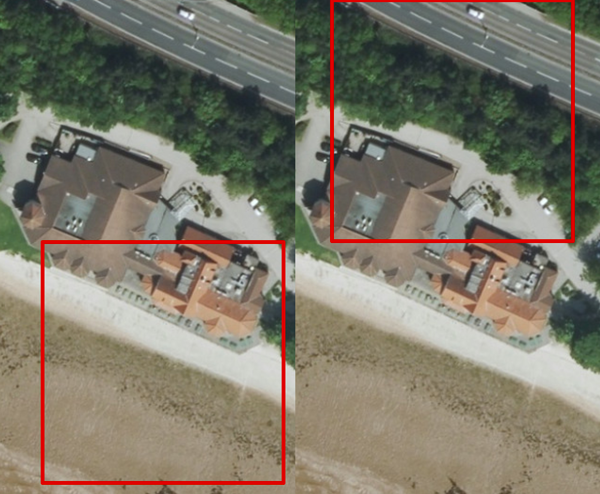
\includegraphics[width=\textwidth]{figs/6/fuzzy-old}
    \caption{With a fixed 256x256px grid, the house that a user wants to select crosses the border of two tiles, so they are unable to select it.}
    \label{fig:prod:fuzzyold}
\end{figure}

To combat this issue, instead of just splitting the image into 256x256px tiles, it was split into 128x128px tiles, and these smaller tiles would act as `selection tiles’ for the larger tiles. The larger tile would contain the smaller `selection tile’ in the top left, with it’s neighbouring tiles filling in the rest of the larger tile. The 128x128px tiles were then used to display the map using Google Maps API, however when selecting one of these tiles, it’s larger counterpart would be the area that actually was selected. This effectively meant that the system moved from a 256x256px selection grid to a 128x128px selection grid whilst maintaining a 256x256px selection size, effectively quadrupling the selection space. With this new system, the user is able to select an area that was previously split between borders of tiles, helping remove fuzzy borders. The result of this as compared to figure \ref{fig:prod:fuzzyold} can be seen below in figure \ref{fig:prod:fuzzynew}.

\begin{figure}[H]
    \centering
    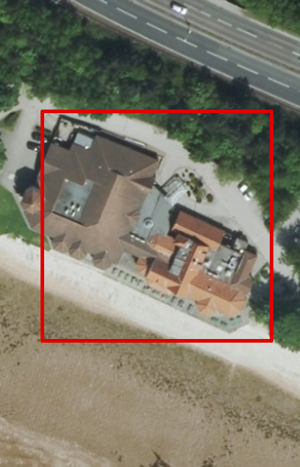
\includegraphics[width=8cm]{figs/6/fuzzy-new}
    \caption{With a 128x128px grid, and 256x256px selection, a user can now select a house that used to lay in the middle of two tiles.}
    \label{fig:prod:fuzzynew}
\end{figure}

\subsection{Learn and Discover Mode}

Having completed the processing of the initial image, Productizer provides two modes to the user: learn and discover. Learn mode provides a method of supervised learning for the classifier, allowing users to select a number of different tiles and a certain class before submitting. These are then sent to Saturn, which in turn provides the classifier with supervised training data generated from these tiles. The classes of the system are displayed in a dropdown, having been retrieved from Saturn, and there is also the ability to add new classes to the system within learn mode. Once the user has finished with learn mode, they are able to switch to discover mode by flipping a simple toggle switch.

Discover mode allows a user to select and filter which class(es) they wish to discover, and markers are added to the map for each tile that matches a selected class, with distinct colours to represent each class. Upon hovering on one of these markers, the class name is also displayed in a simple text bubble. The initial classification is automatically generated upon the initial upload of the image, with every distinct 256x256 tile being sent in batches to Saturn in order to retrieve a classification that is then stored in the database. Every time learn mode is used however, these classifications become outdated, so discover mode also provides the ability to re-classify every tile upon the click of a button, updating this classification data. Storing these classifications inside of a database for each unique tile essentially caches the results, optimising load time.

\subsection{Amazon SQS}

The first design iteration would simply create a GET request containing all of the tile image URLs, and submit this to Saturn manually for reclassification. This proved to be very inefficient as the request size was large, while server processing and thus response time was slow, and if a request was lost due to network issues or some other means, the user could end up waiting a large amount of time for no reason. To combat this, a queue system was implemented within the application that utilised Amazon Web Service’s Simple Queue System (SQS) to store and handle different jobs that were to be completed. In order to handle the retrieval and submission of these tasks, a new task worker, ‘Grunt’, was introduced as explained below. Storing these tasks with SQS meant that a smaller request could be sent to SQS to store the processing data, and then the user could be presented with a processing page until every item in the SQS queue had been processed so that they were aware of what was happening behind the scenes while waiting for their new classifications to be displayed. Furthermore the queue worker enabled retries to be handled if a request fails, delegating responsibility of ensuring the job is completed to the queue worker as opposed to the user. This new implementation greatly boosts user experience.

\subsection{PubNub}

One of the goals with the new processing page was for the user to be informed of the processing results in real time, without the need to constantly refresh the page to check the status of processing. This would mean that, as well as improving user experience, it would reduce server load in the scenario where a user would constantly refresh the page. In order to achieve this goal, a publish-subscribe mechanism was implemented with PubNub. The ‘topic’ used for PubNub would be a unique map ID, allowing the queue worker to publish on to this topic every time a new tile batch had been processed. The Javascript code within the map display page would subscribe to this topic, and every time a message was received informing it that a new batch had been processed, the user interface would be updated to reflect this. This real-time data transfer meant it was possible to display a live loading bar, and iteratively add map markers to discover mode as new tile classifications are received.

\subsection{Grunt}

Grunt, the queue worker, utilises Laravel’s built in job and queue functionality. Out of the box, Laravel enables the use of Amazon SQS as a queue driver, meaning implementation was greatly simplified. In order to create a job type, a specific job class needed to be build, that was named BatchProcessTile. The tile generation process was responsible for defining batches of tiles, and passed through a collection of tiles to each new job. The implementation with SQS operates by serializing the job object once it has been constructed and sending this to Amazon’s servers. Once Grunt retrieves this queue object, it is deserialized and the `handle’ method of the job is called. Within the `handle’ method, the collection of tiles is formed into a request that is sent to Saturn, with a retry handler that takes care of re-sending failed requests. Once an accepted response is retrieved from Saturn, containing the re-classification data, the `handle’ method updates each tile from the batch, storing it’s new classification in the database. Once this has been completed, it publishes a completion message to PubNub as explained above.

The decision to create Grunt as a separate microservice arose early on in project testing when the back-end was not making use of the GPU, so responses took a lot longer to receive than they do in the current iteration of the application. At this stage, Productizer would simply send all requests itself directly to Saturn in order to retrieve the result, which took 5 minutes or more for the response to be received, whilst all the user would see was a white screen with a loading wheel in their browser. This is a dreadful user experience, and from testing it was revealed that users would often refresh during this process, which would reset the waiting time and put more strain on the server. By implementing Grunt, the user was taken to a processing page as soon as the image had been uploaded, so they were informed with exactly what was going on via a loading bar indicating progress. Despite this problem being much less severe now that the back-end makes full use of the GPU, it helps mitigate other potential issues that could have arisen during this process, such as network issues that might have caused a request to be interrupted, putting responsibility on Grunt to complete the task.

\section{Testing} \label{section:prod:testing}

Testing was heavily integrated within the development of Productizer. As the focus during development was heavily based around user experience (UX), the testing was tailored towards this. Functional testing, look and feel testing and usability testing were all carried out to ensure the UX of the application was optimal. 

\subsection{Functional Testing}

The functional testing set out to ensure all buttons/GUI elements behaved as expected. This involved making sure links lead to the correct locations, the correct results were obtained from certain stages of the application, and the overall functionality of the system worked as intended. No formal documentation was created for this testing, as with every new iteration of Productizer, the entire process of the system was tested from the start, meaning that every aspect of the site was checked during each iteration. 

\subsection{Look and Feel Testing}

One key part of optimising UX for the user was the look and feel testing. With this, it was important to ensure that the process of using the application was enjoyable and straightforward. To check this, external feedback was required, so throughout the development lifecycle, colleagues were asked to navigate around and use the application, and provide feedback. Additionally, one fantastic component of scrum was the weekly meetings with Izzy, providing direct UX tests with the client every week, allowing for adjustments to the UI and UX based upon her feedback in time for the next sprint.

The most noticeable change to the UX that arose from look and feel testing was the migration from using a small area for the map with the controls down the side, as shown in figure \ref{fig:prod:olddesign}, to having a much larger full width map, with the controls underneath, as shown in \ref{fig:prod:newdesign}. One colleague had a much larger resolution display compared to the devices used for development. With this, they identified a problem where workflow could potentially be slowed due to such a restrictive map area. Following this feedback, a full screen map layout was developed, and other colleagues and Izzy were asked which layout they preferred. The result was unanimous in favour of the fullscreen layout, so this became the new design.


\begin{figure}[H]
    \centering
    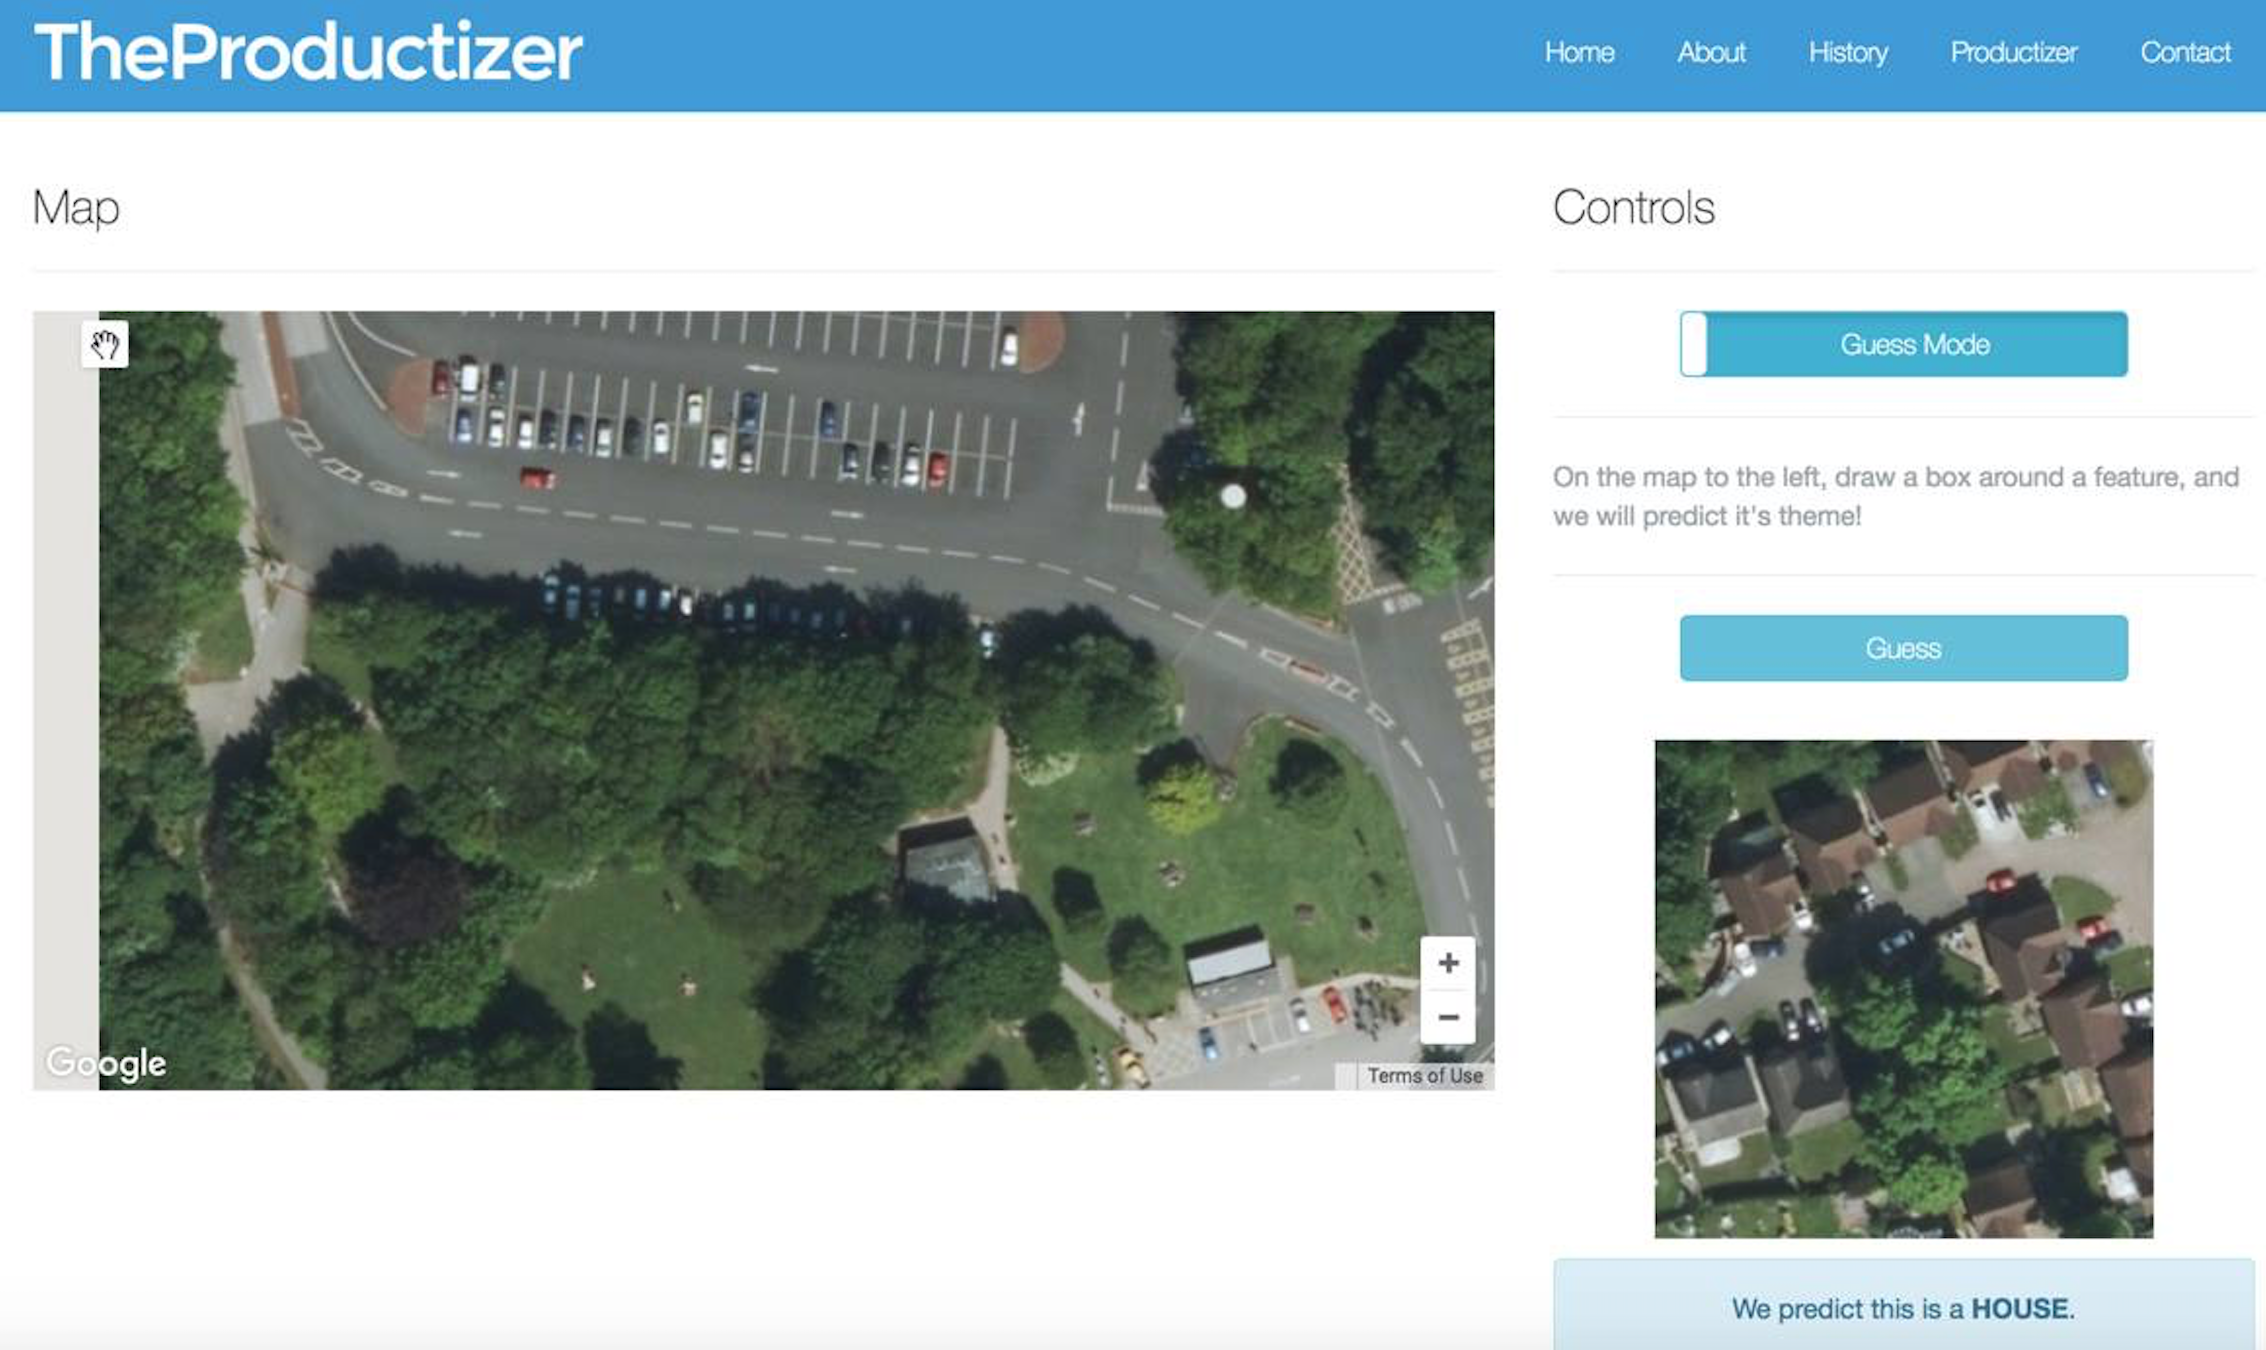
\includegraphics[width=\textwidth]{figs/6/6-testing-olddesign}
    \caption{The initial Productizer design, with small map interface and controls along the side.}
    \label{fig:prod:olddesign}
\end{figure}

\begin{figure}[H]
    \centering
    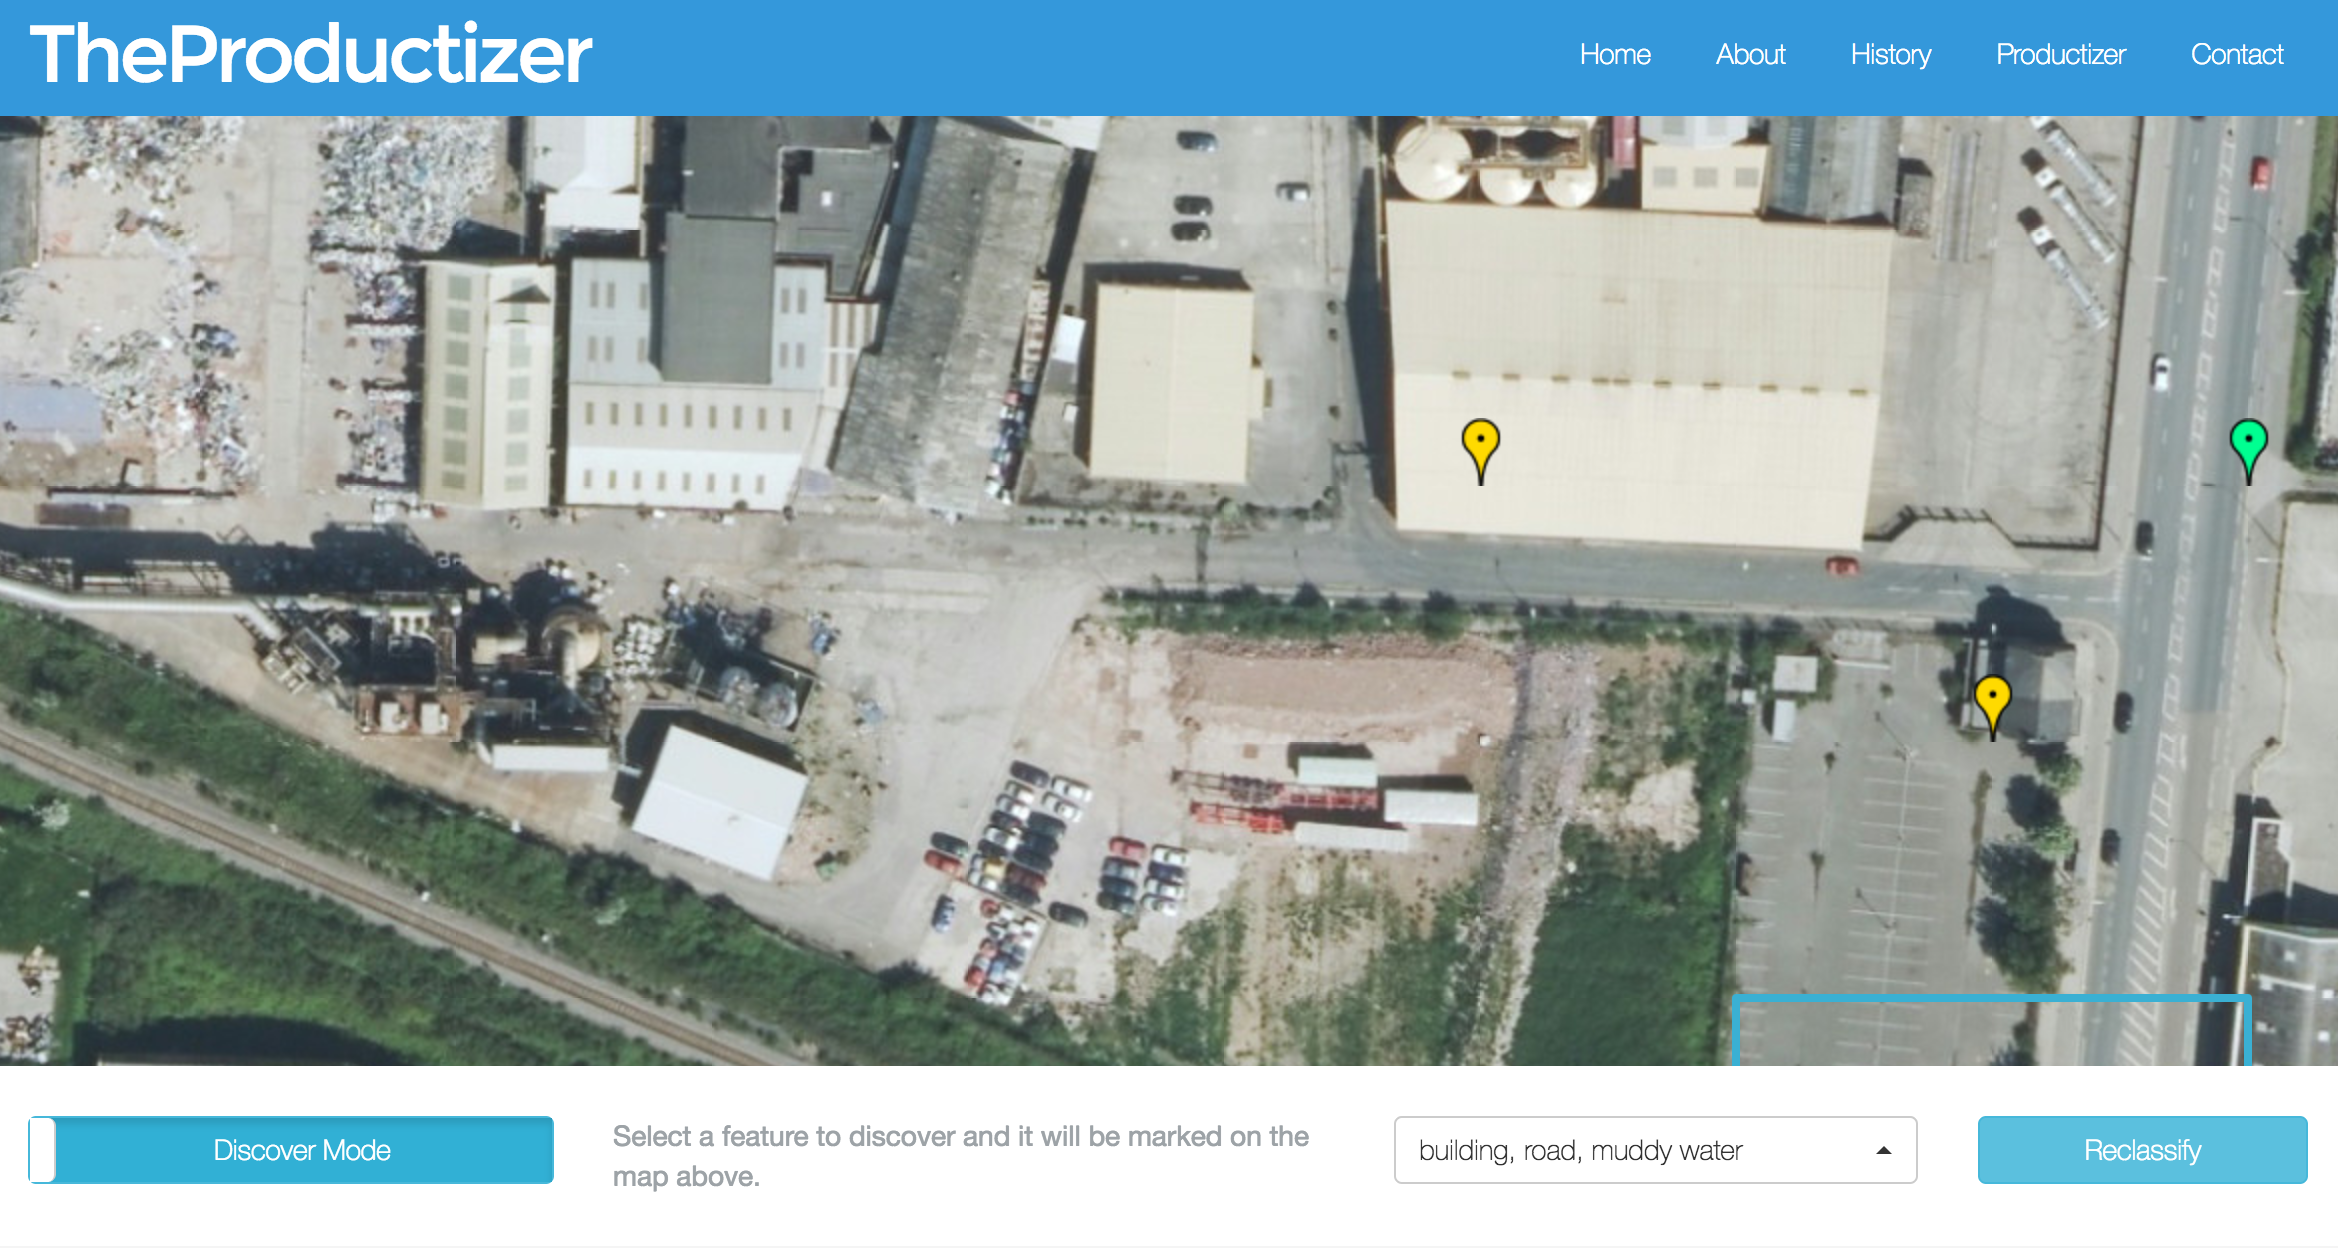
\includegraphics[width=\textwidth]{figs/6/6-testing-newdesign}
    \caption{The revised Productizer design, with full width map interface and controls along the bottom.}
    \label{fig:prod:newdesign}
\end{figure}



\subsection{Usability Testing} \label{section:productizer:usability}

Usability testing involves sitting a user down with the system and running them through a specific process to test ease-of-use and identify confusing features or features that could be improved.

As mentioned in the above implementation, one issue identified early on during usability testing was the initial loading time during the uploading and processing of the image due to the communication to Saturn, that could take anywhere up to 5 minutes or beyond. Upon identifying this problem, research was carried out into typical response times and their effects on the human brain. \cite{nielsen_1993} found that a 0.1 second response was considered an “instantaneous response”, a one second response was the limit of maintaining a user’s flow of thought, and ten seconds was the limit of keeping the user’s attention. This article also stated that in a situation where instantaneous feedback cannot be provided to the user, a “percentage-done” indicator should be used. The original plan was to optimise the loading time to be within this 10 second limit of attention, however within the time constraints of the project this was not a viable aim, so a “percentage-done” indicator was implemented as suggested, and can be seen below in figure \ref{fig:prod:loading}.


\begin{figure}[H]
    \centering
    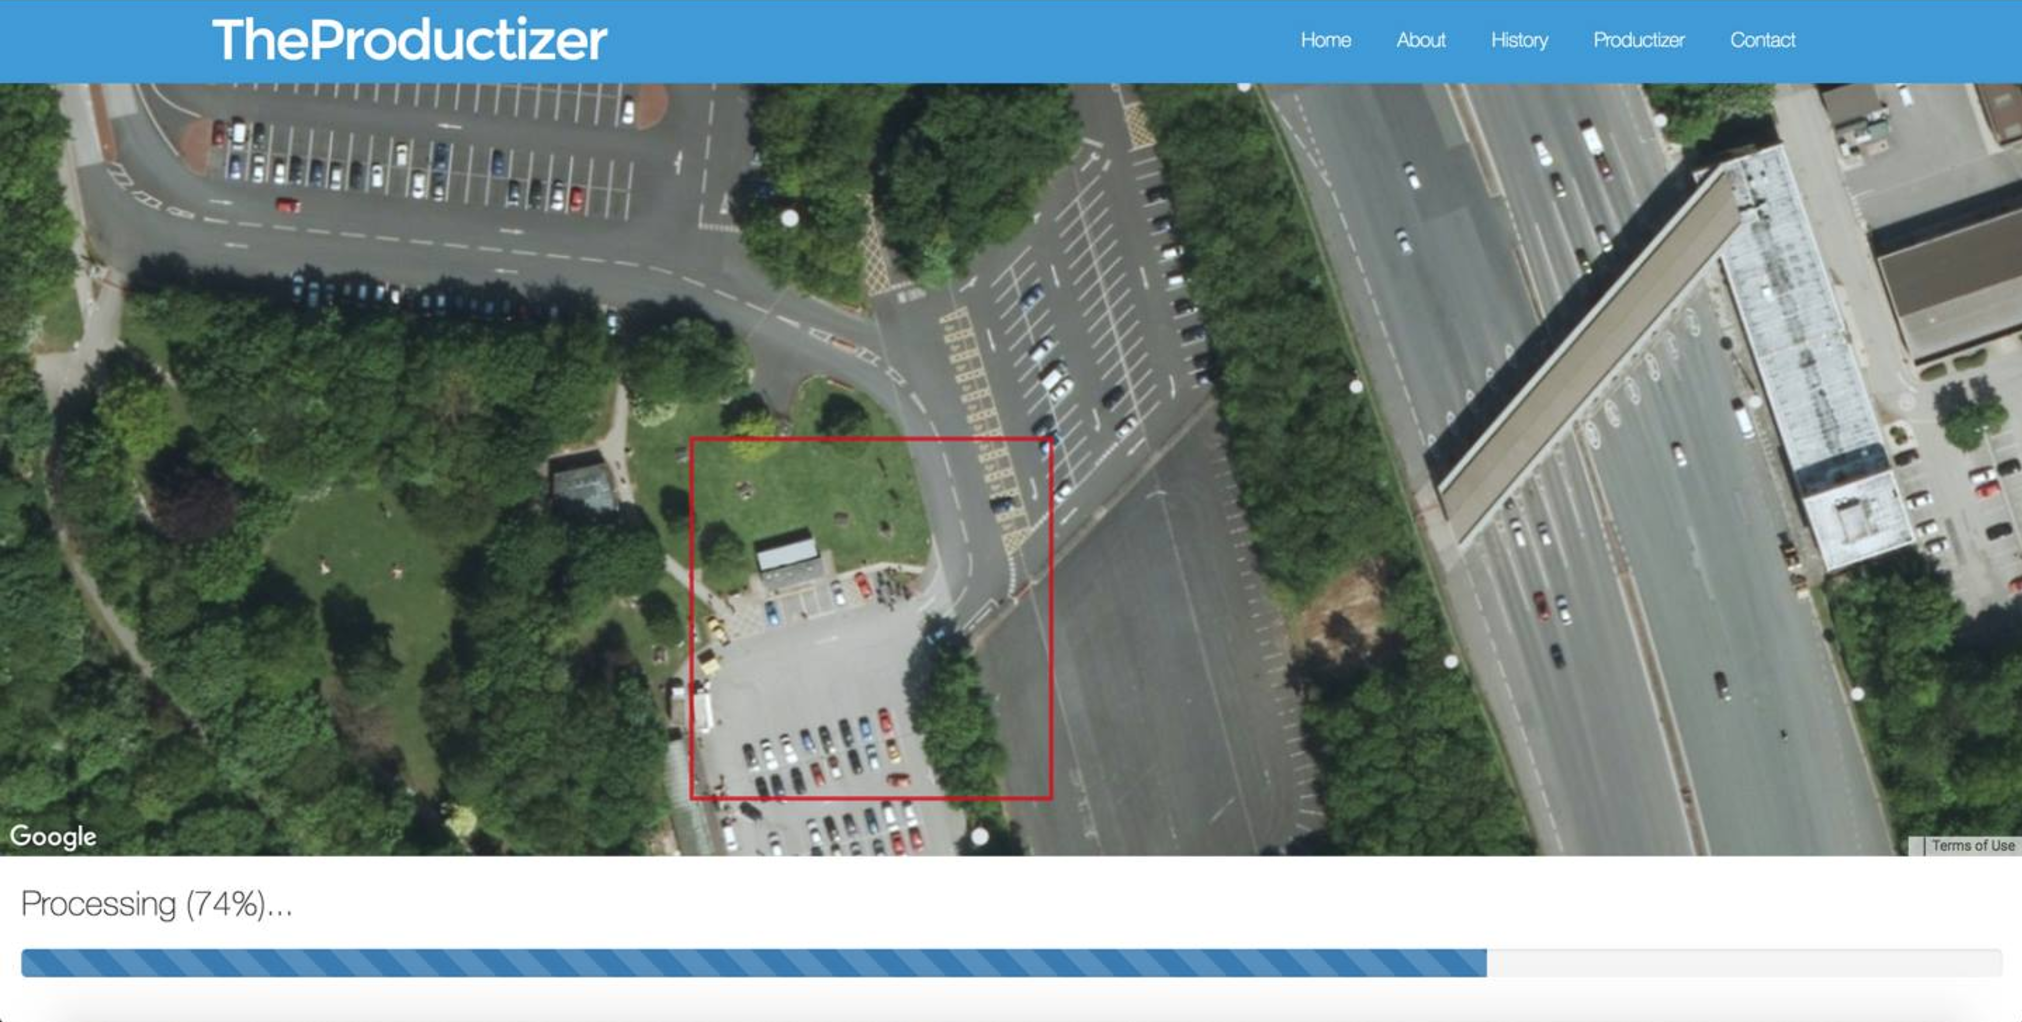
\includegraphics[width=\textwidth]{figs/6/6-usability-loading}
    \caption{A percentage-based loading indicator provides the user feedback of processing percentage.}
    \label{fig:prod:loading}
\end{figure}

Final results of the usability testing conducted with Ordnance Survey can be seen in the results section further on in this report in section \ref{chapter:results}.

\section{Limitations}

A limitation found during testing Productizer was the time that it takes for a user to upload an image to the system. Most sample images provided by Ordnance Survey were around 40 to 50MB in size, and these images could take a significant time to upload if the user’s upload speed was slow, and lead to additional issues should the user’s network be unstable. Unfortunately this is an external limitation that cannot easily be optimised within the scope of this project. However, the images provided by Ordnance Survey were of TIFF format which, when converted to JPEG, were much smaller in size (around 4 to 5MB) without significant loss in quality, so it may be quicker to convert the TIFF images to JPEG format before upload, should the user have a slow connection.

\section{Evaluation}

The user-facing web application, Productizer, was designed to be a solution that allows a user to upload an aerial image and, through a streamlined process, manipulate and select regions on a map in order to train a classifier, and obtain its predictions to discover features similar to those used in training. Following the three required features of the web application outlined at the start, Productizer is now a complete solution for this design, with a heavy focus on optimising the user experience through this process. A user can upload an image, and can then select a number of different tiles to be used to teach the system. Following this, they can use “Discover Mode” in order to identify and filter different features identified on the image that they have uploaded. The design is mobile-optimized too, allowing for flexibility in its use across multiple devices.